
\chapter{Litt om Overleaf}\label{kap:overleaf}


Dette kapittelet gir en introduksjon til Overleaf i form av en rekke
skjermdump og beskrivende figurtekster.


\begin{figure}[H]
  \centering
  \scalebox{0.35}{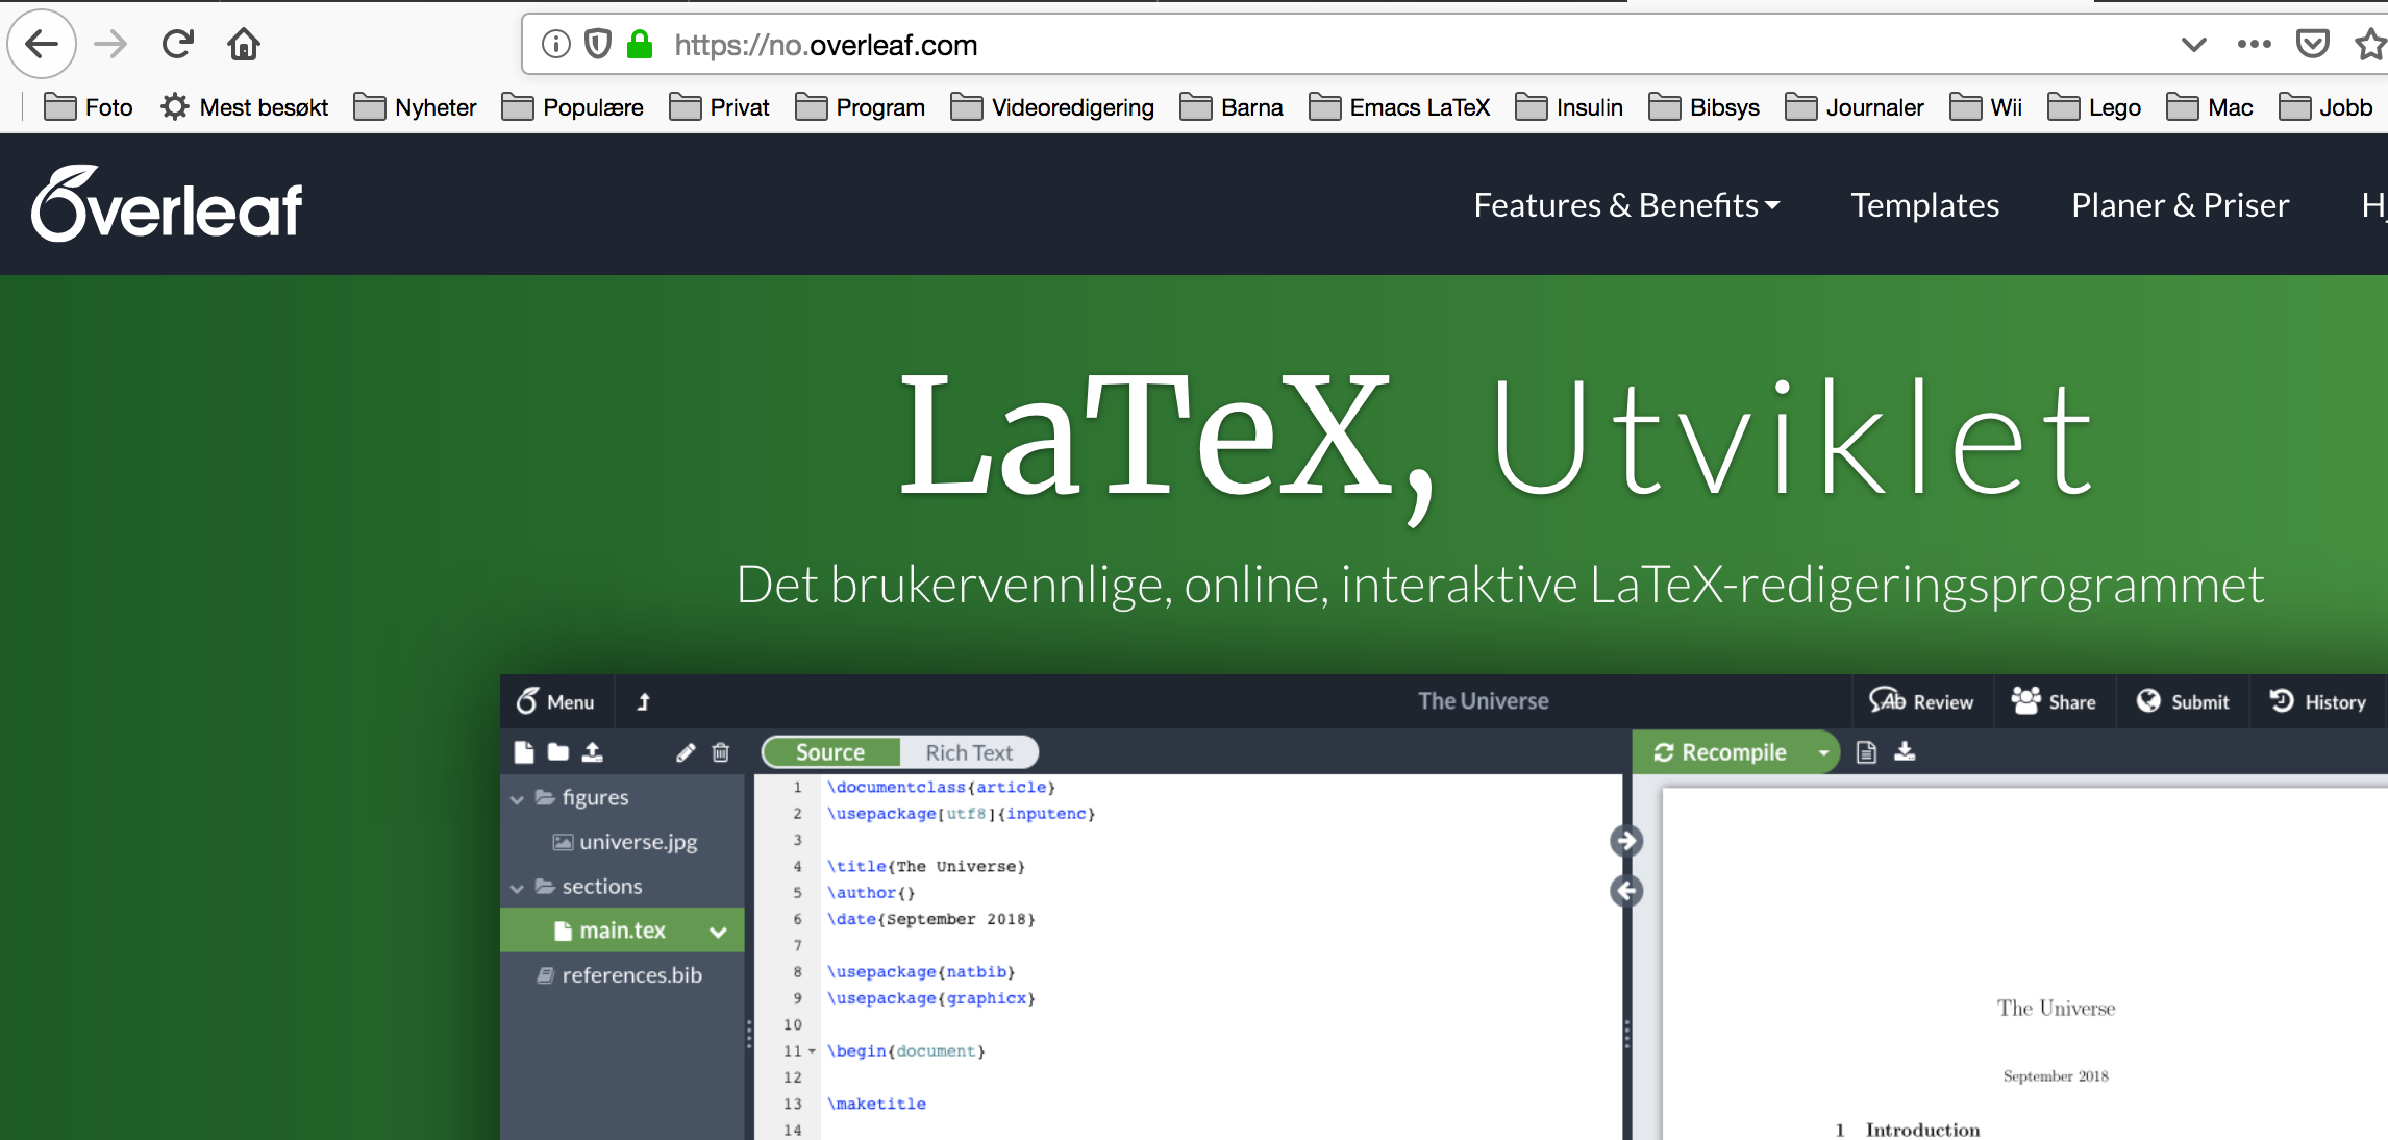
\includegraphics{bilde0}}
  \caption{Gå inn på
    {\color{blue}\href{https://no.overleaf.com/}{https://no.overleaf.com/}}. Registrer
  deg med UiS-epostadressen din. } 
  \label{fig:bilde0}
\end{figure}

\begin{figure}[H]
  \centering
  \scalebox{0.6}{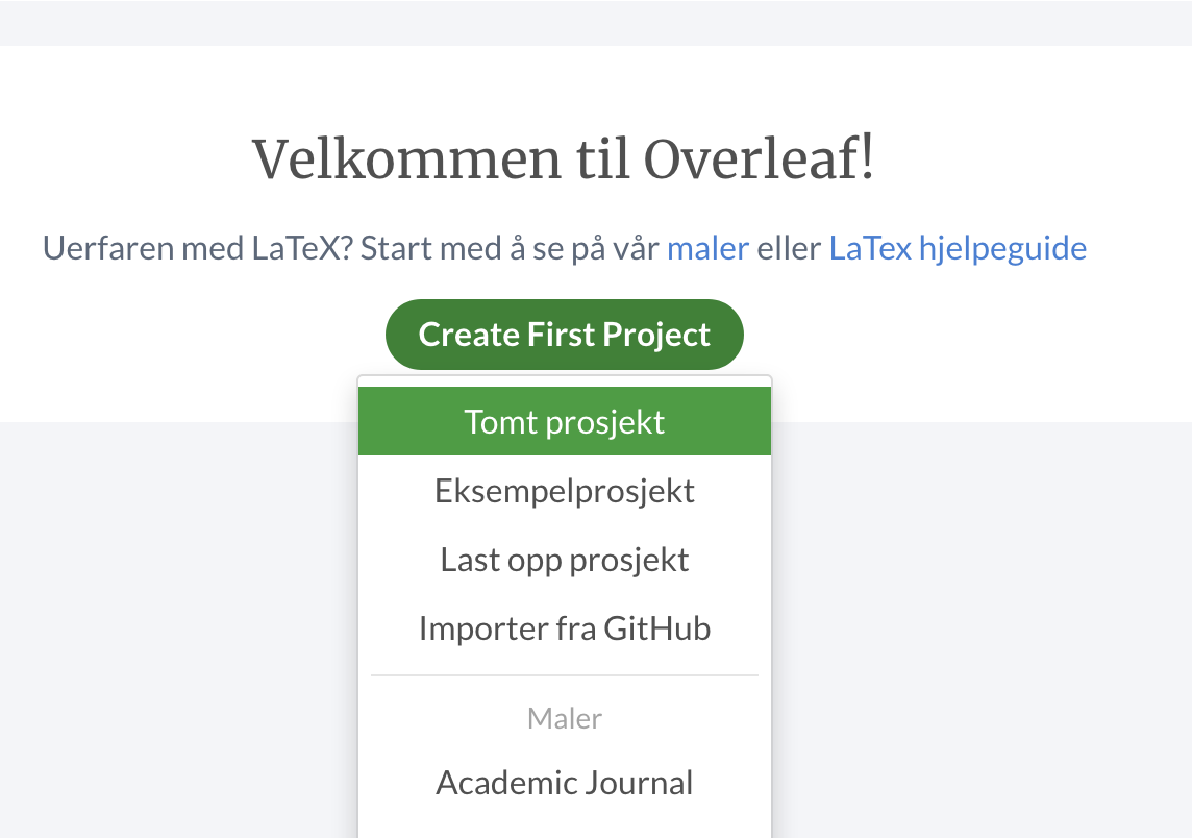
\includegraphics{bilde1}}
  \caption{Etter at du har registrert deg og logget deg inn, trykk på
    ``Create First Project'' og velg ``Tomt prosjekt''.}  
  \label{fig:bilde1}
\end{figure}

\begin{figure}[H]
  \centering
  \scalebox{0.5}{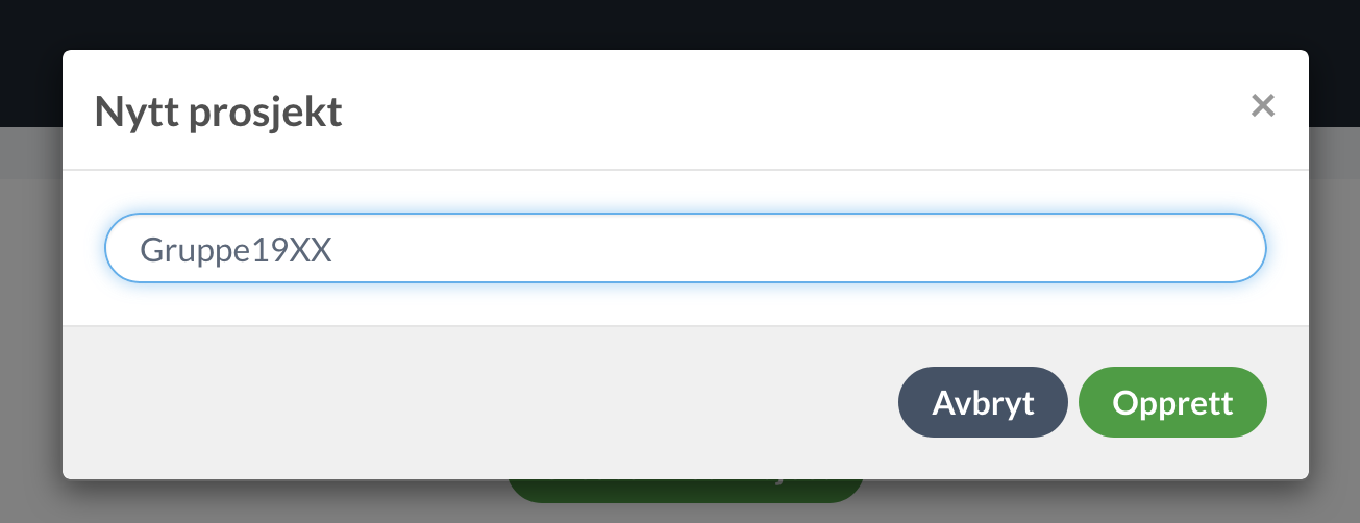
\includegraphics{bilde2}}
  \caption{Kall prosjektet ``Gruppe19XX'' hvor XX er
    gruppernummeret deres.} 
  \label{fig:bilde2}
\end{figure}

\begin{figure}[H]
  \centering
  \scalebox{0.6}{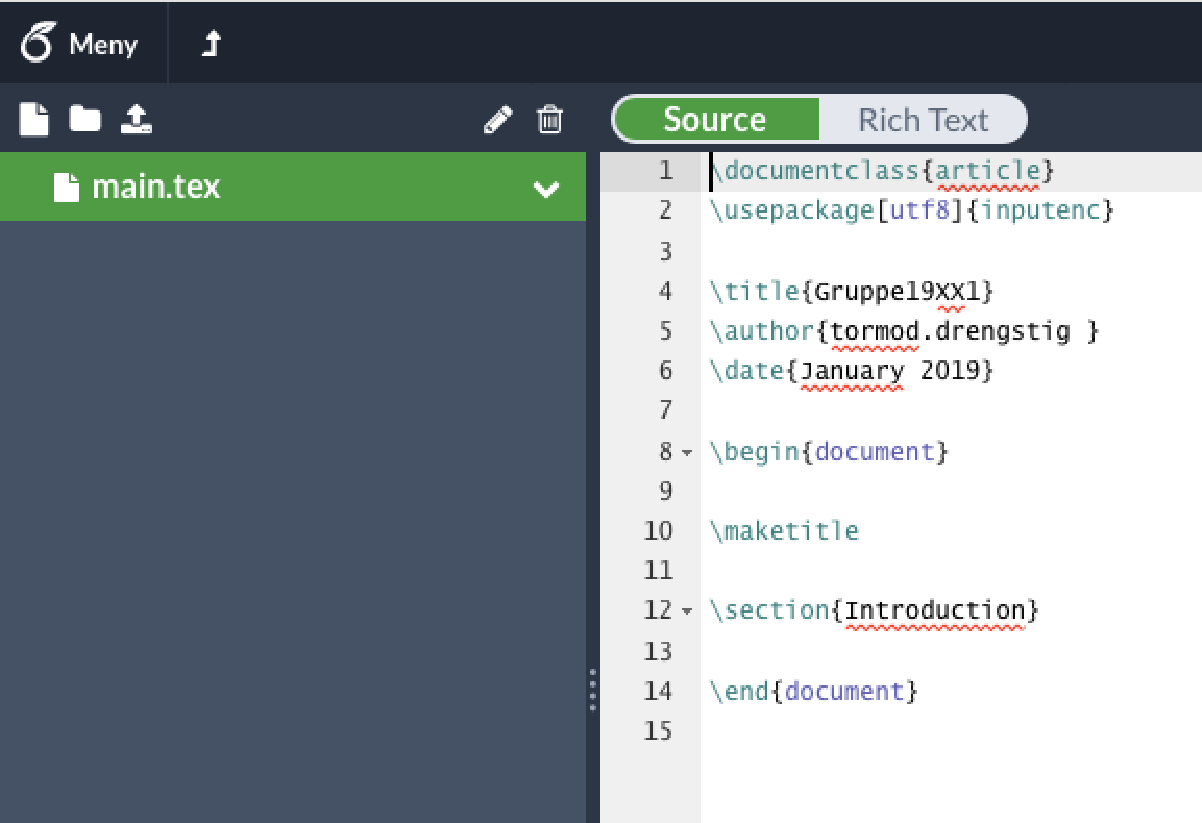
\includegraphics{bilde2a}}
  \caption{Det opprettes automatisk opp en hovedfil kalt 
    \fbox{\tt main.tex} i prosjektet.} 
  \label{fig:bilde2a}
\end{figure}

\begin{figure}[H]
  \centering
  \scalebox{0.8}{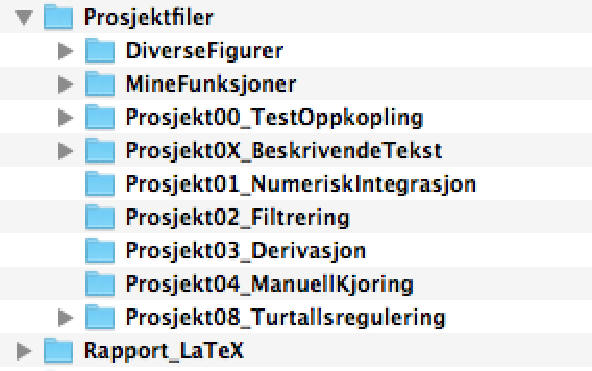
\includegraphics{bilde2b}}
  \caption{Nå er poenget at mappestrukturen som er å finne i {\tt
      Lego.zip}-filen skal lages i Overleaf-prosjektet. Vær klar over
    at det i mappen \fbox{DiverseFigurer} ligger endel figurer samt \fbox{\tt
      overleaf}-mappen. } 
  \label{fig:bilde2b}
\end{figure}

\begin{figure}[H]
  \centering
  \scalebox{0.6}{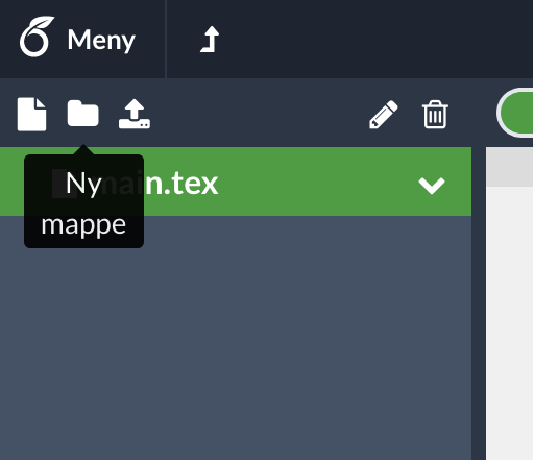
\includegraphics{bilde4}}
  \caption{Trykk på symbolet ``Ny mappe''.} 
  \label{fig:bilde4}
\end{figure}

\begin{figure}[H]
  \centering
  \scalebox{0.6}{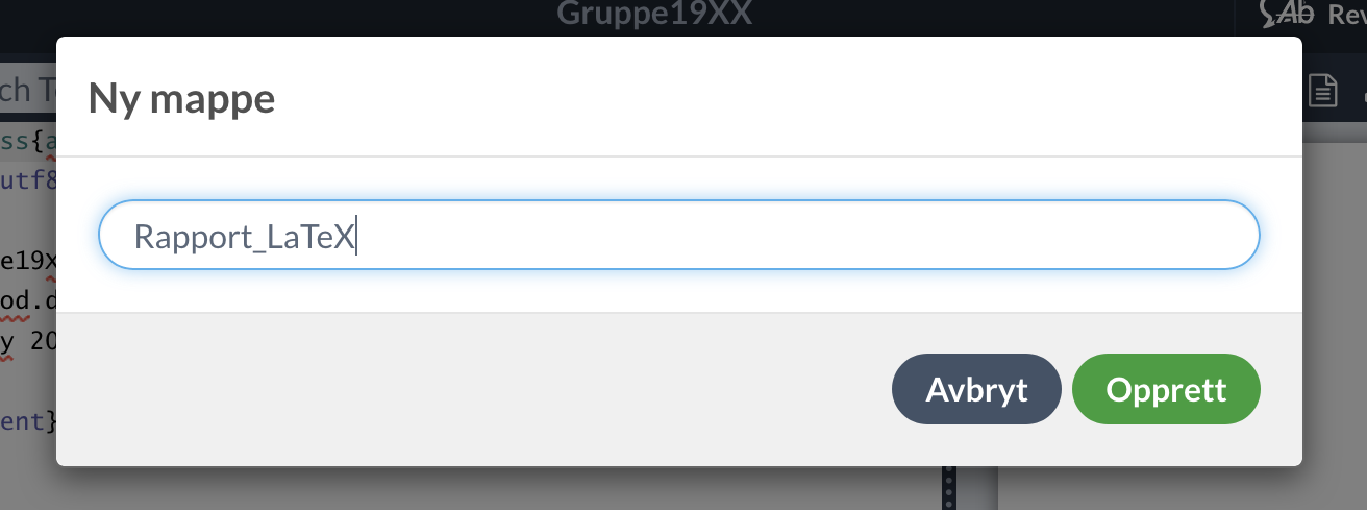
\includegraphics{bilde5}}
  \caption{Lag mappen \fbox{Rapport\_LaTeX}.} 
  \label{fig:bilde5}
\end{figure}


\begin{figure}[H]
  \centering
  \scalebox{0.6}{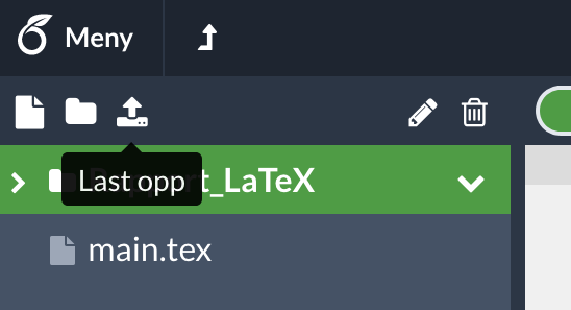
\includegraphics{bilde6}}
  \caption{Stå i mappen \fbox{Rapport\_LaTeX} og trykk ``Last opp''.} 
  \label{fig:bilde6}
\end{figure}


\begin{figure}[H]
  \centering
  \scalebox{0.4}{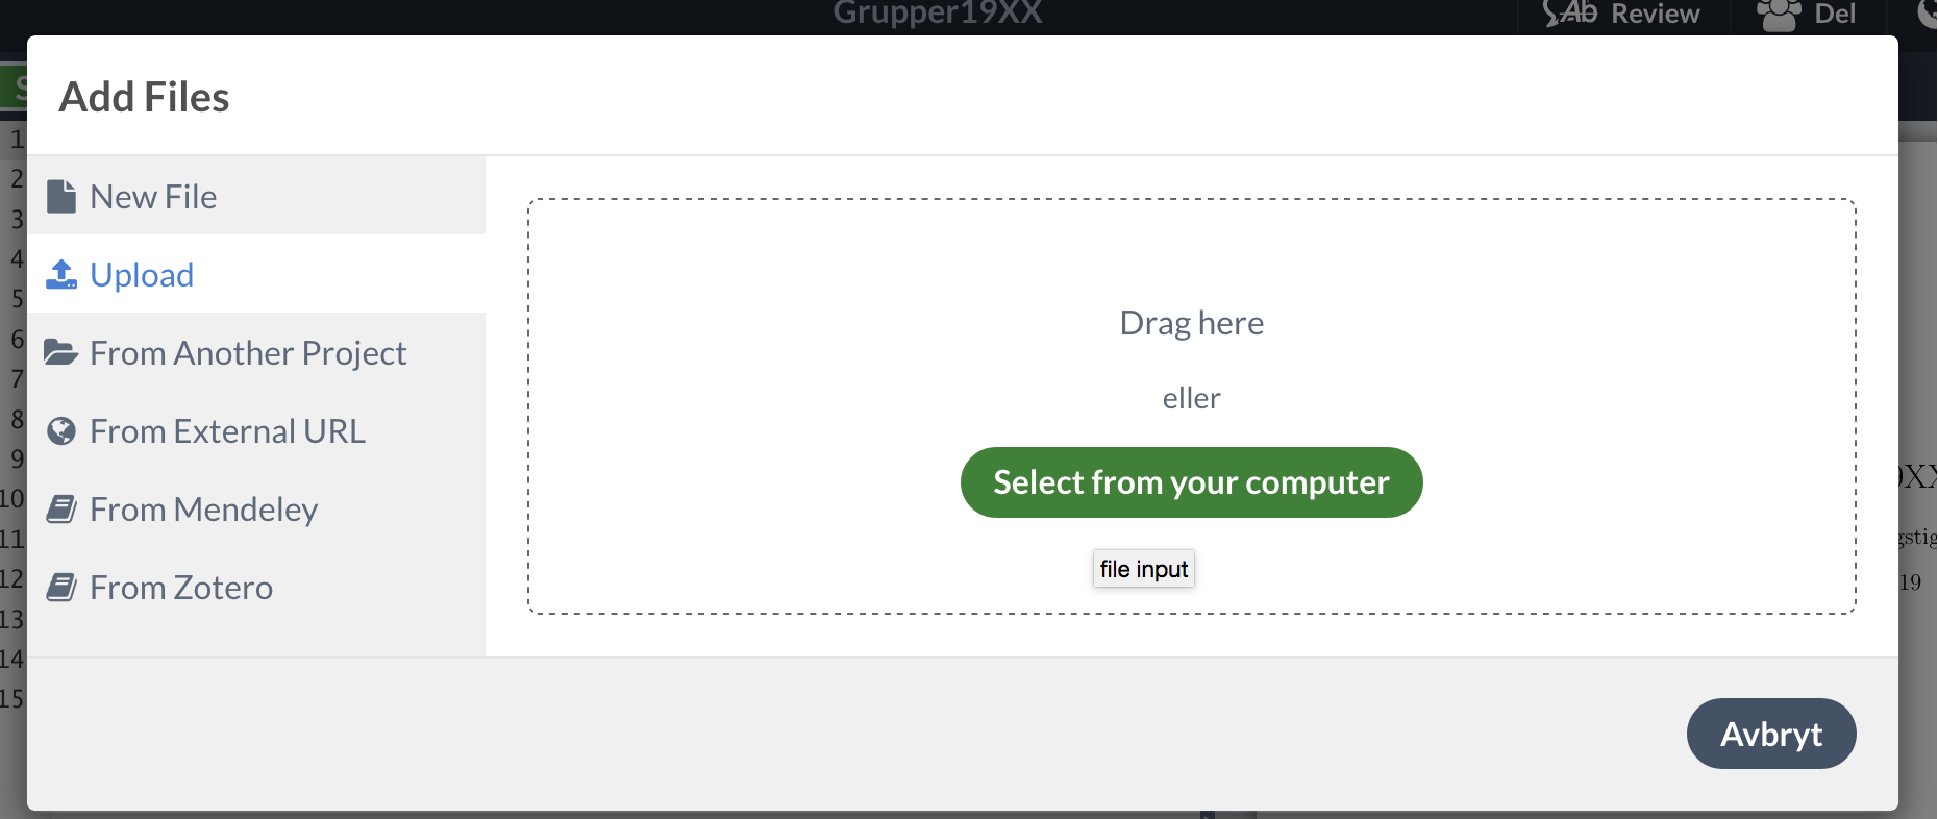
\includegraphics{bilde7}}
  \caption{Trykk på ``Select from your computer''.} 
  \label{fig:bilde7}
\end{figure}

\begin{figure}[H]
  \centering
  \scalebox{0.6}{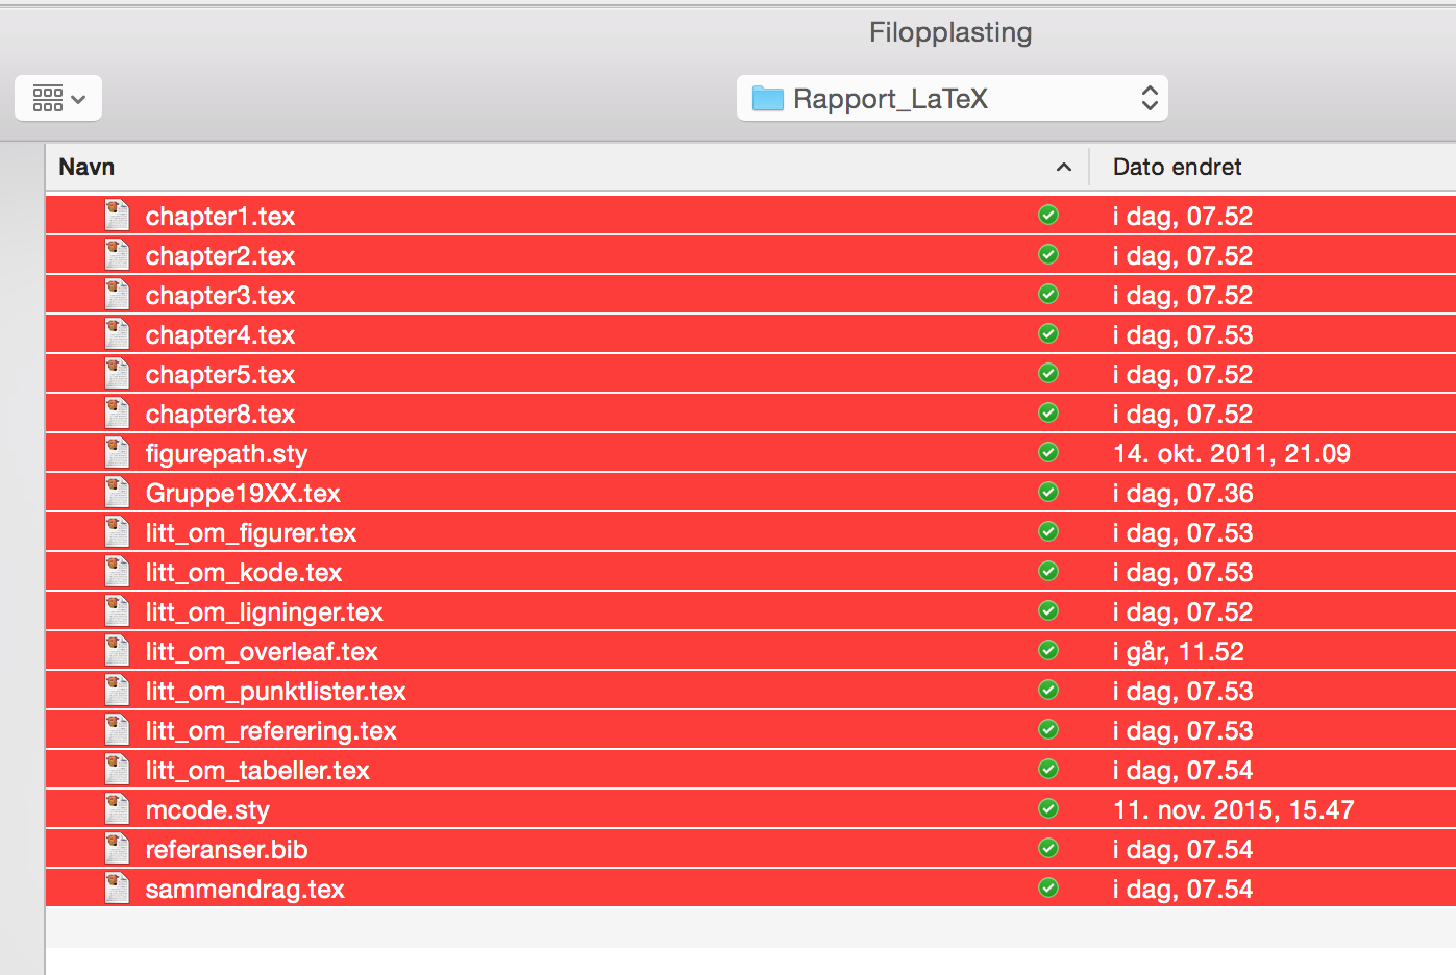
\includegraphics{bilde8}}
  \caption{Naviger deg frem til mappen \fbox{\tt Rapport\_LaTeX} og velg alle filene.} 
  \label{fig:bilde8}
\end{figure}


\begin{figure}[H]
  \centering
  \scalebox{0.4}{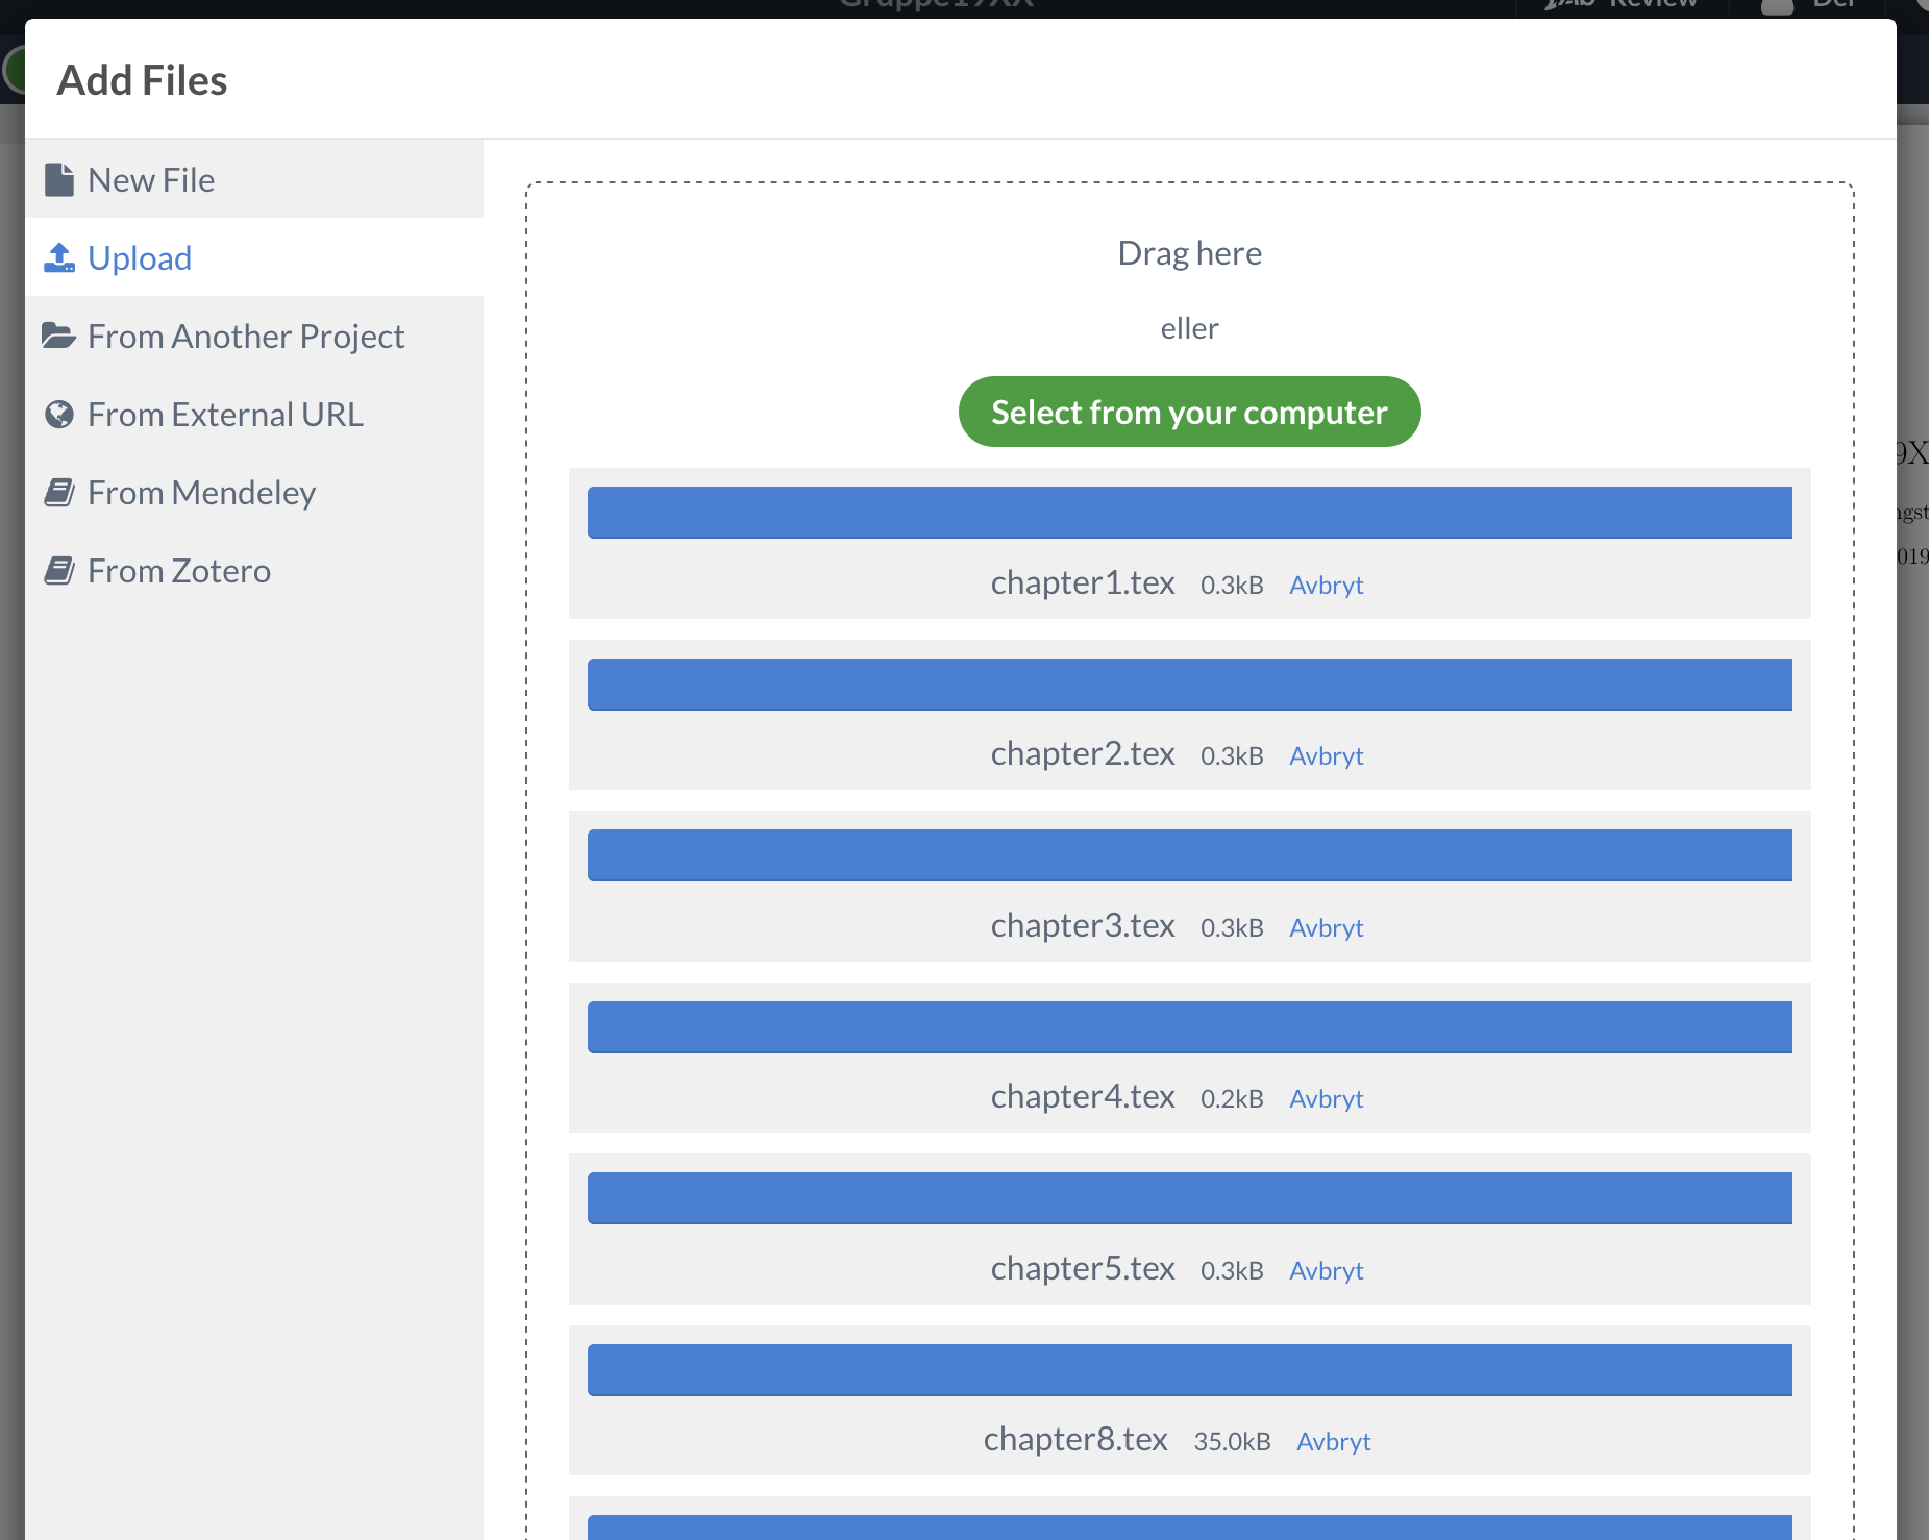
\includegraphics{bilde9}}
  \caption{Filene lastes inn.} 
  \label{fig:bilde9}
\end{figure}


\begin{figure}[H]
  \centering
  \scalebox{0.5}{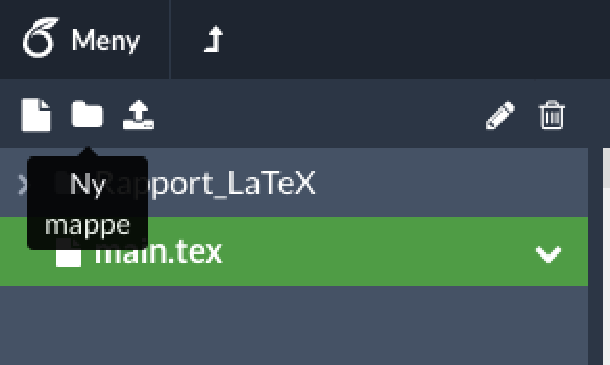
\includegraphics{bilde10}}
  \caption{Stå i filen \fbox{\tt main.tex}, og trykk ``Ny mappe'', og lag
    på samme måte som vist i figur~\ref{fig:bilde5} den nye 
    mappen \fbox{\tt Prosjektfiler}.} 
  \label{fig:bilde10}
\end{figure}

\begin{figure}[H]
  \centering
  \scalebox{0.55}{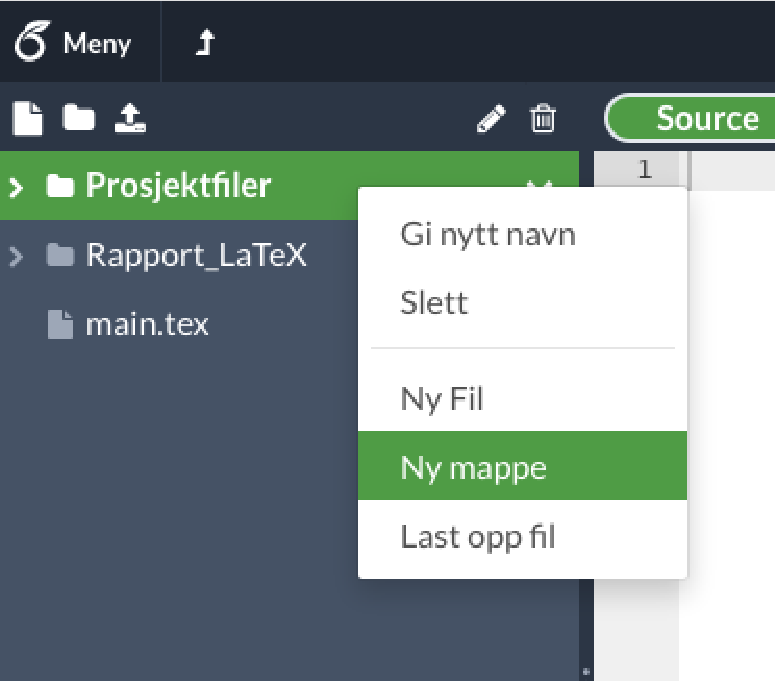
\includegraphics{bilde11}}
  \caption{For å lage undermappene vist i figur~\ref{fig:bilde2b}, 
    stå i mappen \fbox{\tt
      Prosjektfiler}, høyreklikk, og velg ``Ny mappe''. Lag på denne
    måten alle
    mappene som er vist i figur~\ref{fig:bilde12}.} 
  \label{fig:bilde11}
\end{figure}

\begin{figure}[H]
  \centering
  \scalebox{0.55}{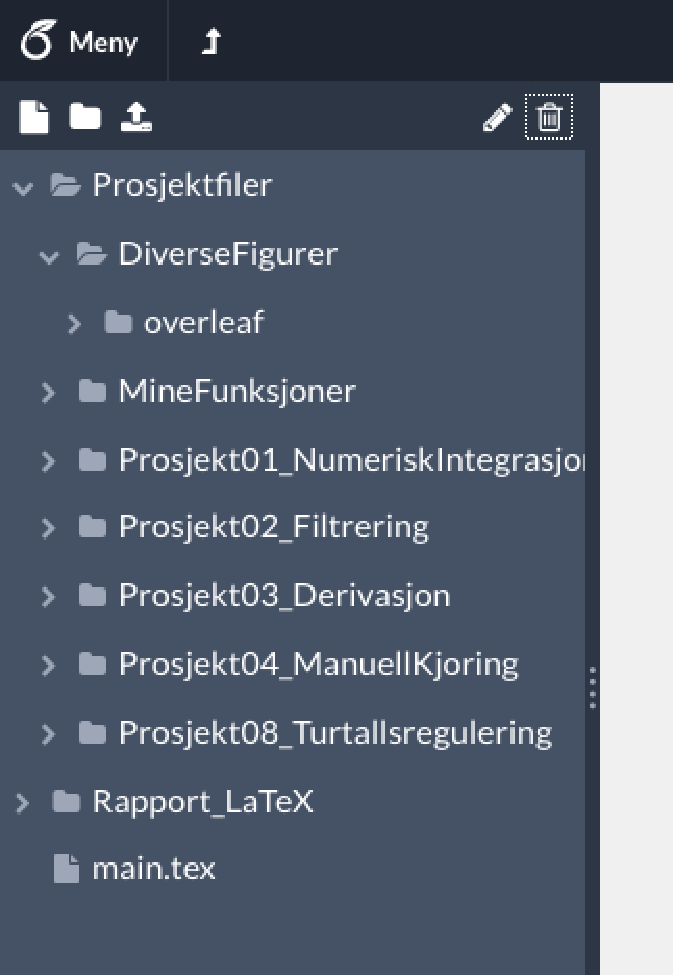
\includegraphics{bilde12}}
  \caption{Mappestrukturen klar.} 
  \label{fig:bilde12}
\end{figure}

\begin{figure}[H]
  \centering
  \scalebox{0.6}{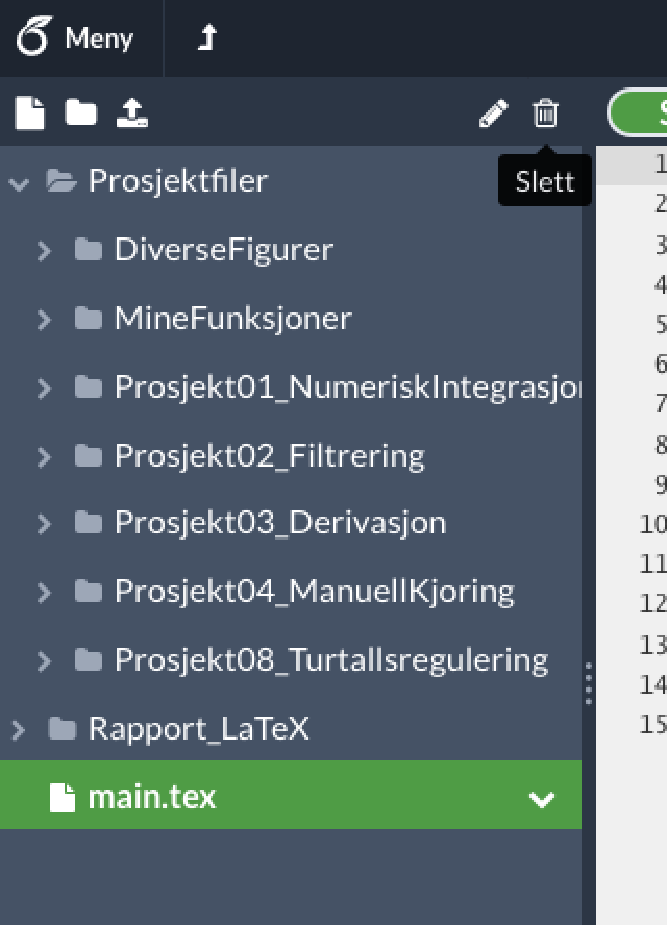
\includegraphics{bilde14}}
  \caption{Slett filen \fbox{\tt main.tex}.} 
  \label{fig:bilde14}
\end{figure}

\begin{figure}[H]
  \centering
  \scalebox{0.7}{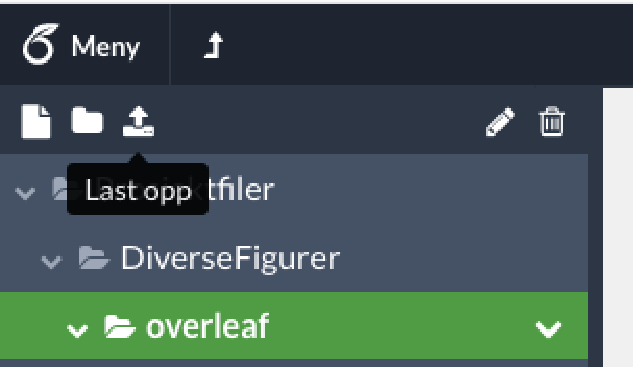
\includegraphics{bilde13}}
  \caption{Nå skal filene i hver mappe lastes inn på samme måte
    som vist i figurene~\ref{fig:bilde6} - \ref{fig:bilde9}. 
    Start f.eks. med å stå i mappen \fbox{\tt overleaf} og trykk ``Last opp''.} 
  \label{fig:bilde13}
\end{figure}

\begin{figure}[H]
  \centering
  \vspace*{-30mm}\scalebox{0.46}{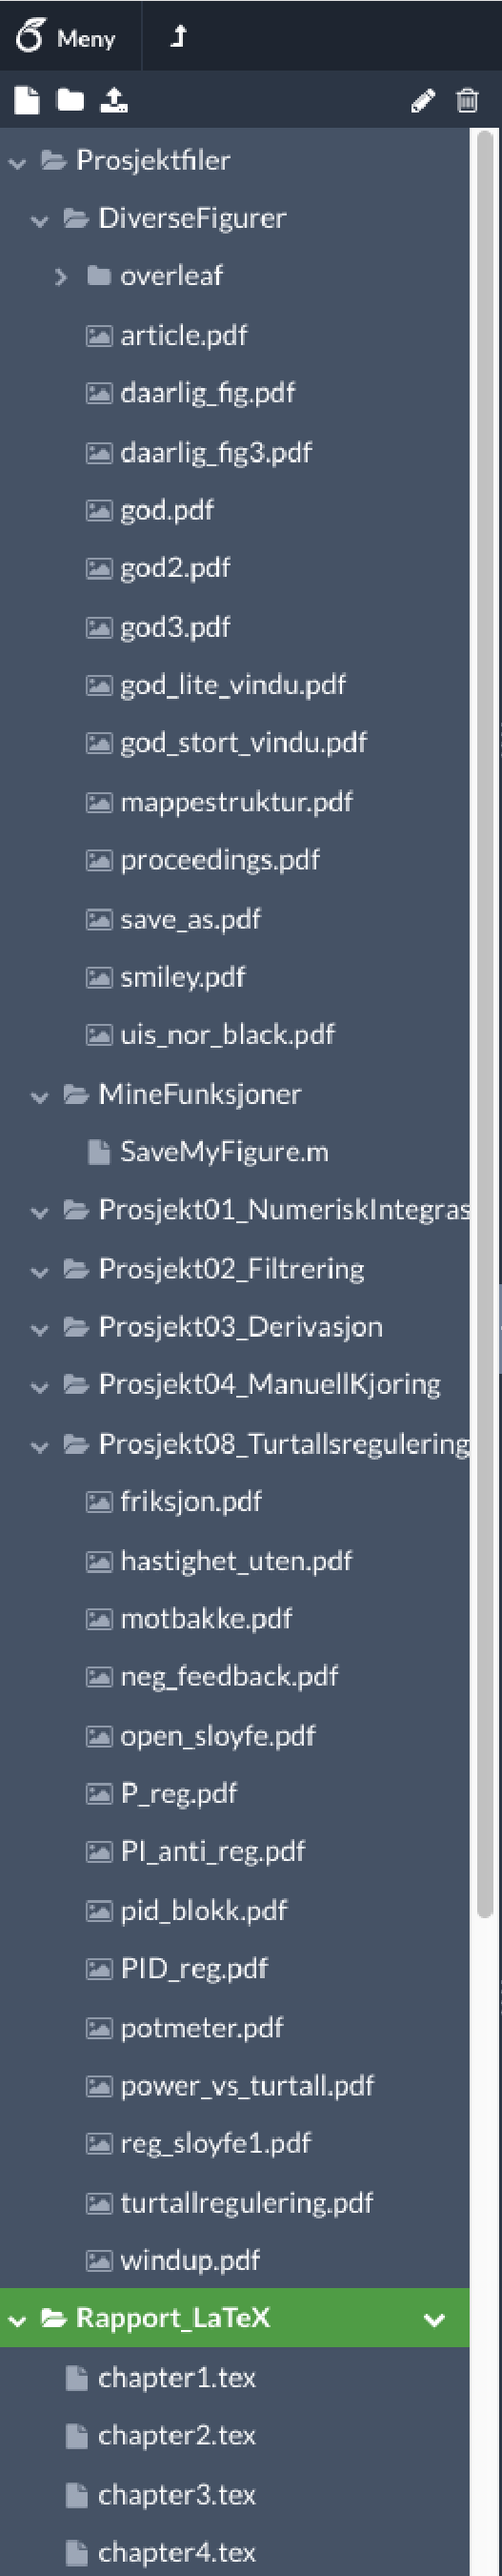
\includegraphics{bilde13a}}
  \caption{Alle filene er på plass. Legg merke til at
    filene i mappen \fbox{\tt overleaf} ikke vises, at mappene
    Prosjekt01... - Prosjekt04... er tomme, samt at det kun er filen {\tt
      SaveMFyFigure.m} som foreløpig ligger i mappen {\tt MineFunksjoner}.} 
  \label{fig:bilde13a}
\end{figure}


\begin{figure}[H]
  \centering
   \hspace*{-30mm}\scalebox{0.6}{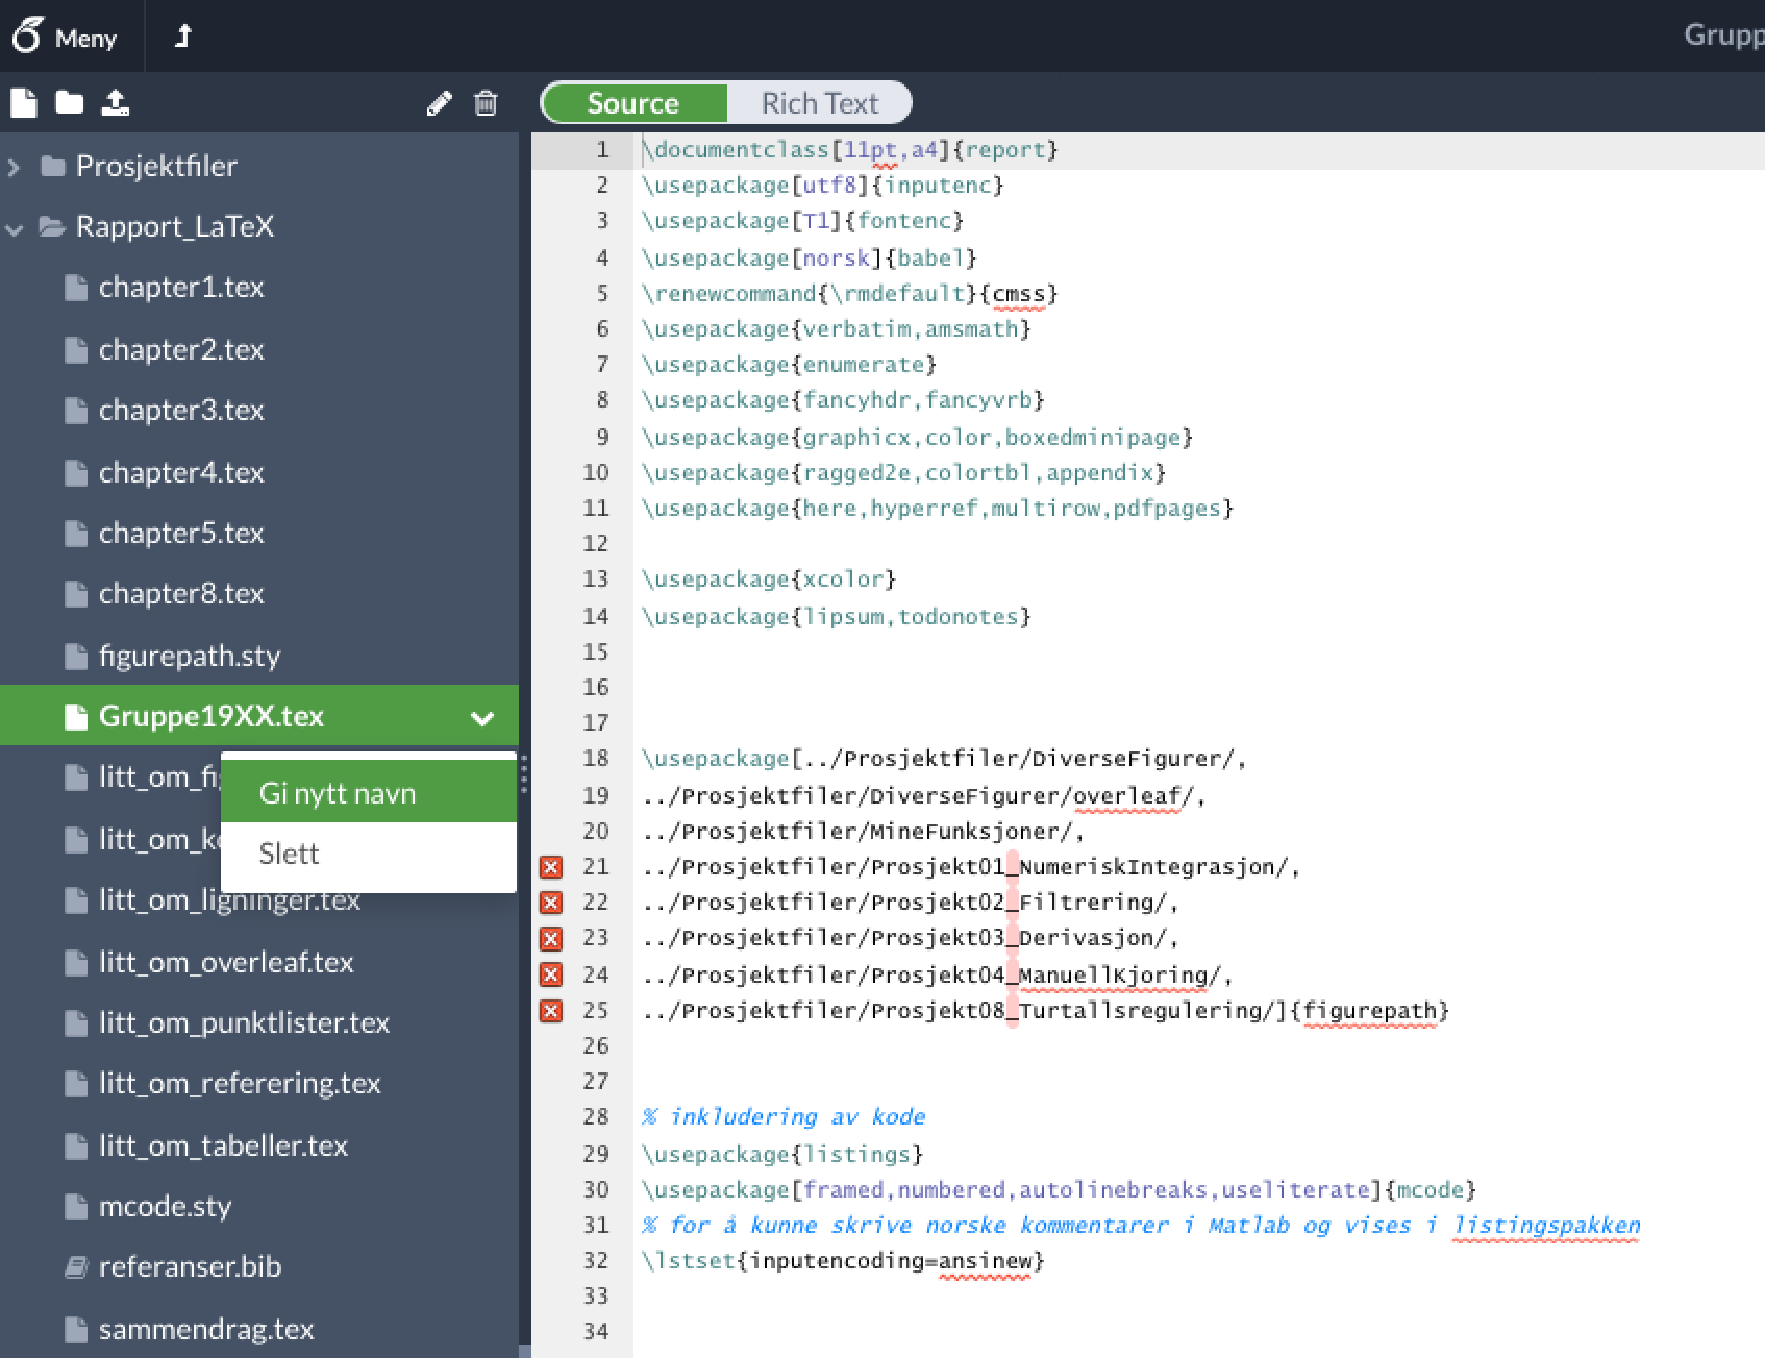
\includegraphics{bilde15}}
  \caption{Trykk på \fbox{\tt Gruppe19XX.tex}. Høyreklikk på denne og
    endre navn til gruppenummeret deres.} 
  \label{fig:bilde15}
\end{figure}

\begin{figure}[H]
  \centering
 \scalebox{0.6}{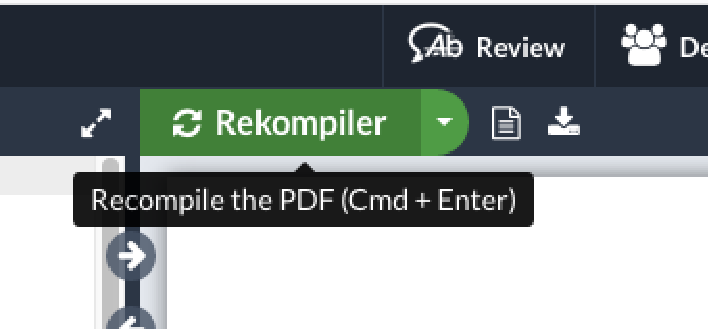
\includegraphics{bilde16}}
  \caption{Trykk på knappen hvor det står ``Rekompiler''. } 
  \label{fig:bilde16}
\end{figure}

\begin{figure}[H]
  \centering
  \scalebox{0.65}{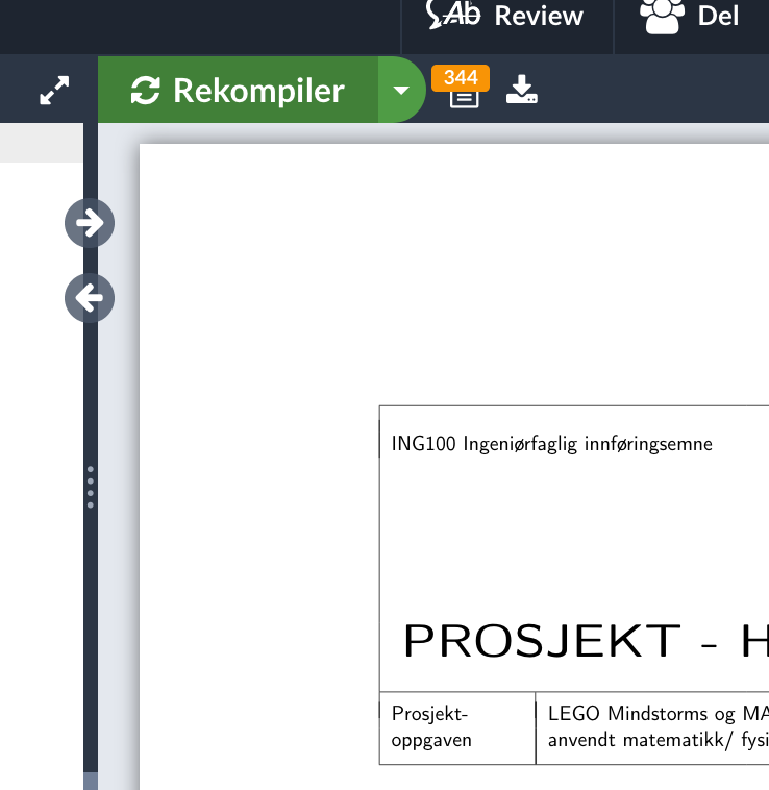
\includegraphics{bilde17}}
  \caption{Etter en stund er den ferdig med å kompilere. Som du ser står det et tall med
    oransje bakgrunn. Det betyr at det er {\em warnings} i
    kompilering. Disse er ufarlige. Dersom bakgrunnen skifter
    farge til {\color{red}rødt} er det kompileringsfeil, og disse må rettes
    opp. Trykk på selve tallet så kommer kompileringsresultatet opp og
    du kan se fra henvisning til linjenummer hvor feilen er.} 
  \label{fig:bilde17}
\end{figure}

\begin{figure}[H]
  \centering
  \scalebox{0.7}{
\includegraphics{bilde18}}
  \caption{For å legge til medstudenter i prosjektet, trykk først på
    pilen med knekk for å komme opp til prosjektsiden.} 
  \label{fig:bilde18}
\end{figure}

\begin{figure}[H]
  \centering
  \scalebox{0.6}{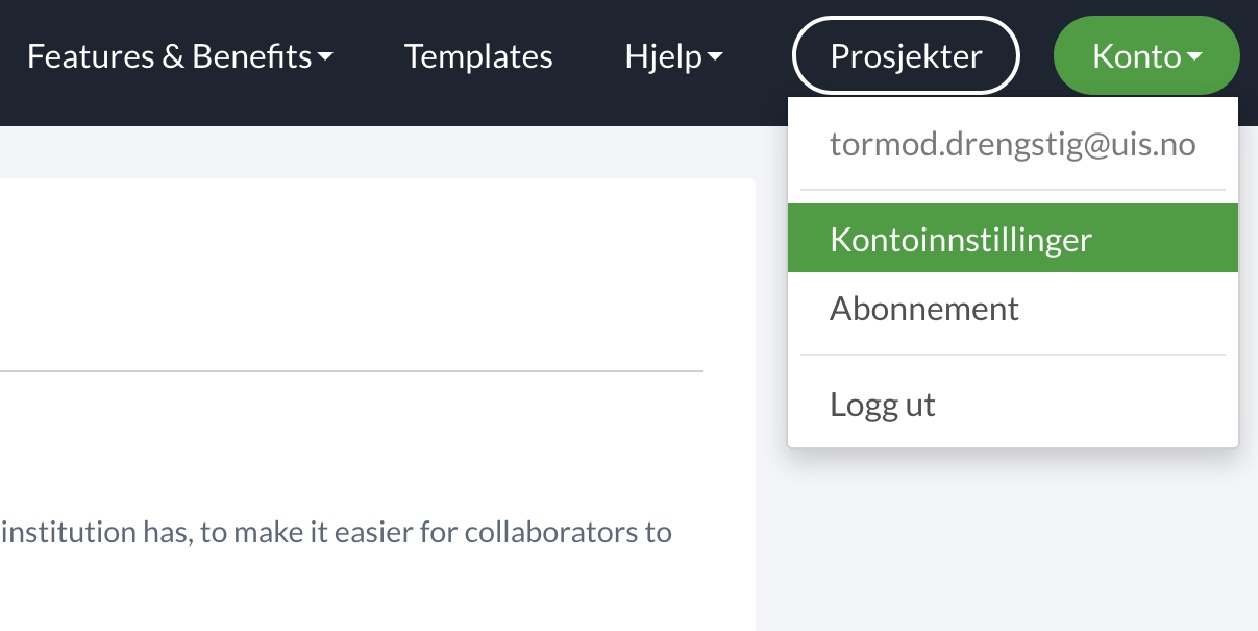
\includegraphics{bilde19}}
  \caption{Trykk deretter på ``Konto'' og ``Kontoinnstillinger''.} 
  \label{fig:bilde19}
\end{figure}


\begin{figure}[H]
  \centering
  \scalebox{0.5}{
\includegraphics{bilde20}}
  \caption{Trykk på ``Featres \& Benefits'' og så ``For Groups''.} 
  \label{fig:bilde20}
\end{figure}


\begin{figure}[H]
  \centering
  \scalebox{0.5}{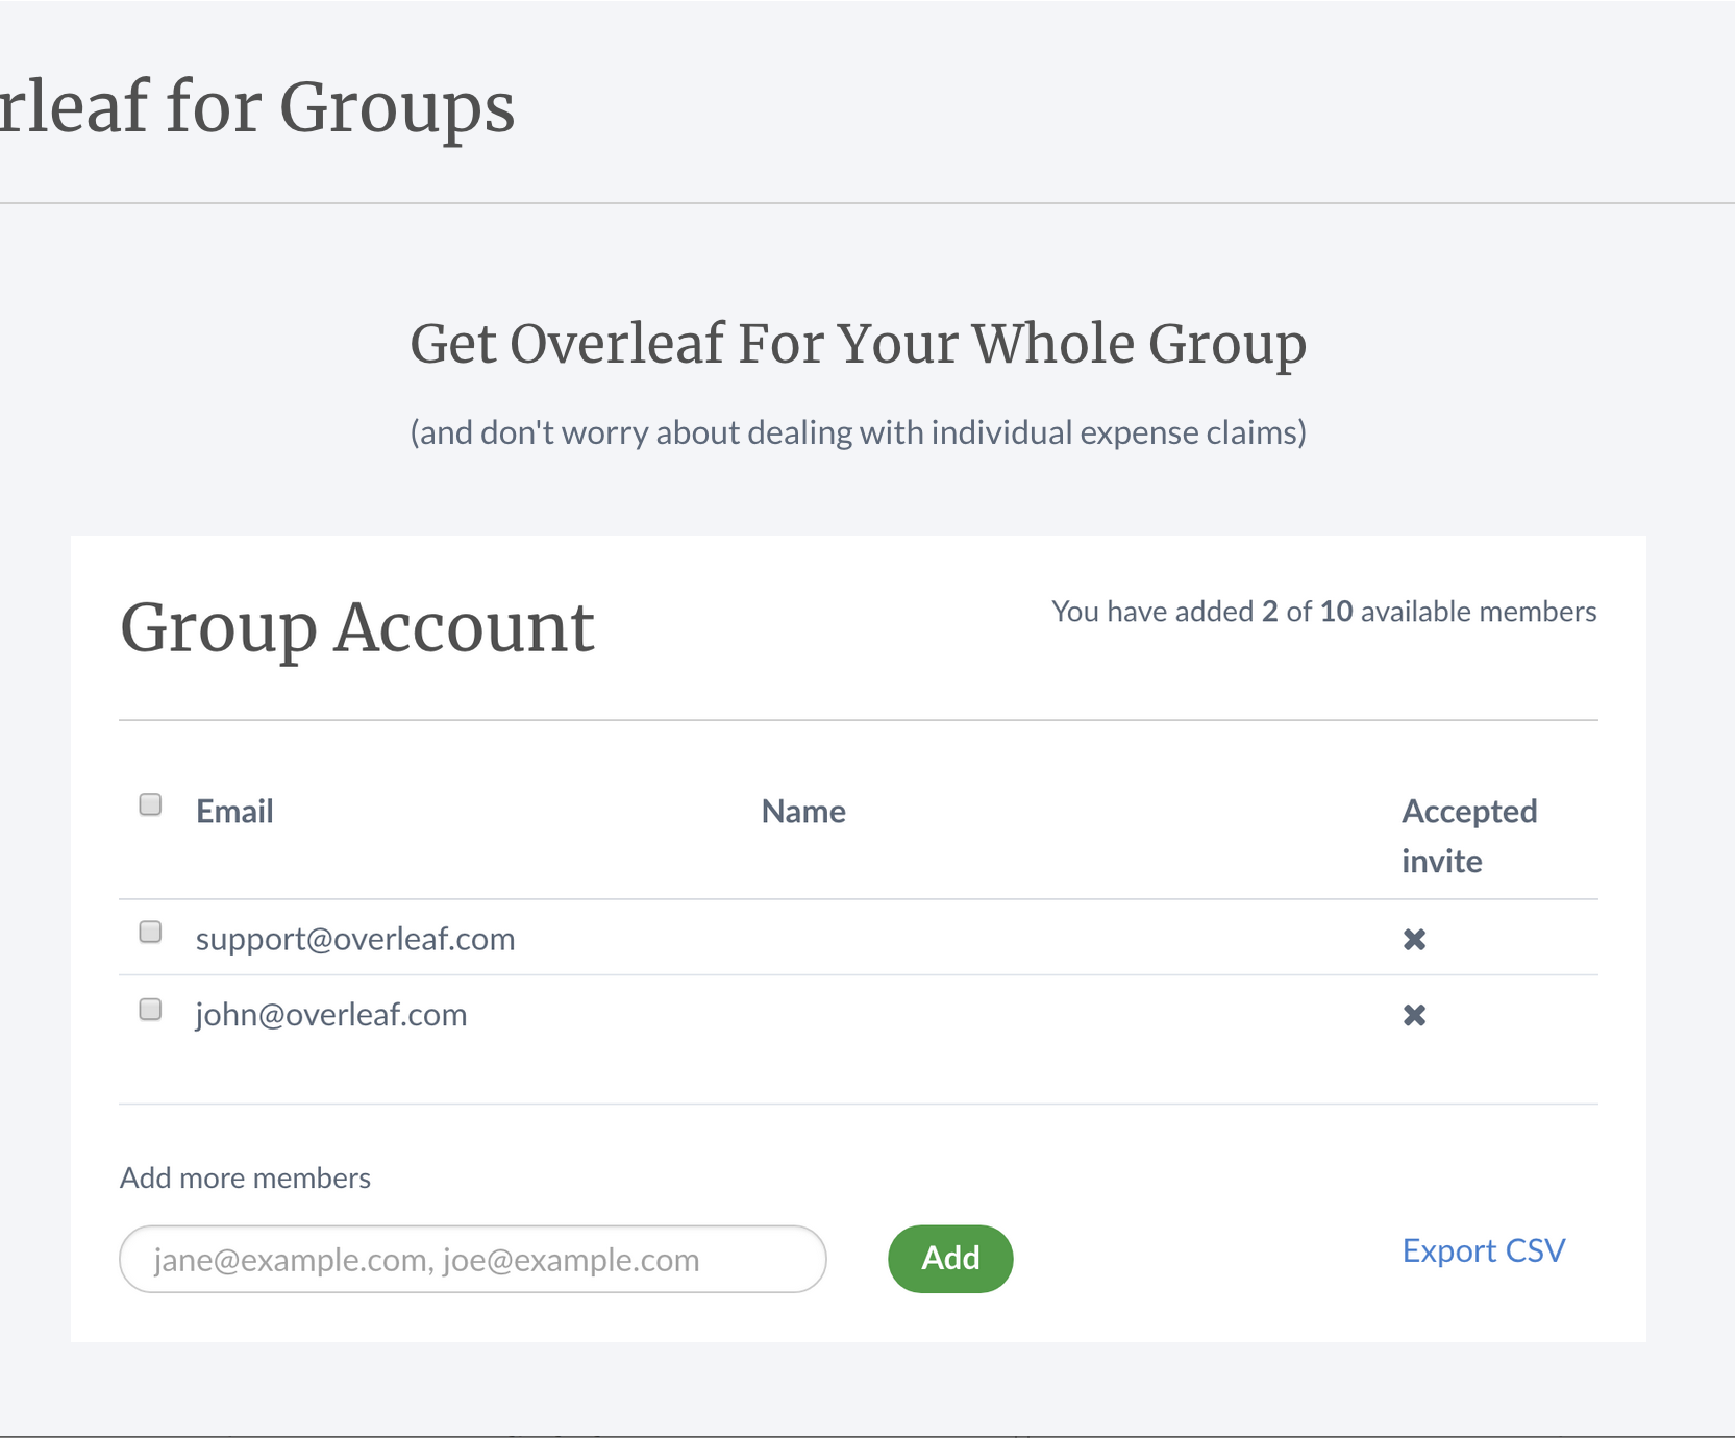
\includegraphics{bilde21}}
  \caption{Legg til studenter med sin registrerte epostadresse
    (UiS-adressen). Disclaimer: Jeg er noe usikker på dette
    her siden jeg ikke har hatt mulighet til å teste det ut.} 
  \label{fig:bilde21}
\end{figure}




